\subsection{Магнитные свойства сэндвичных соединений}

Многие магнитные свойства можно предсказать из МО для большинства металлов. Все электроны спарены – диамагнитная молекула, есть неспаренные – парамагнитная.

\begin{figure}[H]
\centering
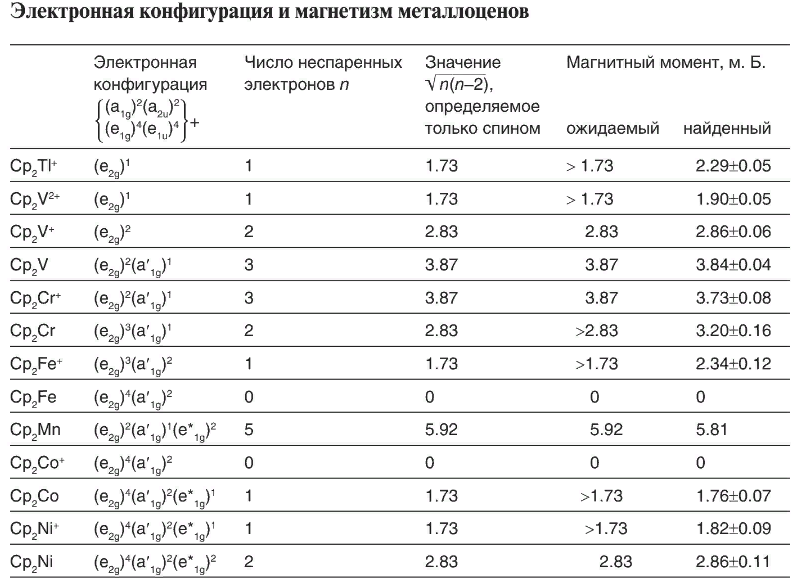
\includegraphics[scale=.600]{images/metallocenes_magn.png}
\end{figure}


Манганоцен в кристалле образует цепи без индивидуальных сэндвичевых молекул. При выше 432 К имеет магнитный момент 5.9 м.Б., что соответсвует электронной конфигурации $(e_{2g})^2 (a_{1g})^1 (e_{1g}^*)^2$ , Декаметилманганоцен $Cp_2Mn$ имеет «нормальную» сэндвичевую структуру и магнитный момент  = 2,18 м. Б. (конфигурация основного состояния $(e_{2g})^2 (a_{1g}^*)^1$ , соответствует низкому спину). Диметилманганоцен состоит из смеси высокого и низкого спинов.

\begin{figure}[H]
\centering
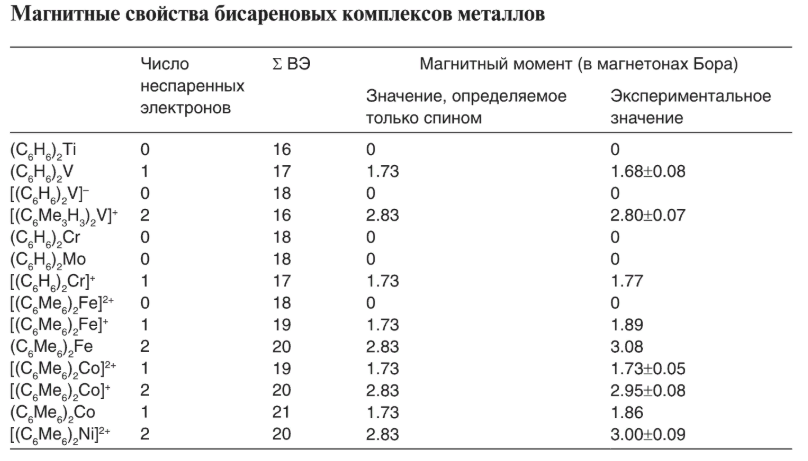
\includegraphics[scale=.600]{images/arenocenes_magn.png}
\end{figure}
